\begin{refsection}
\chapter{Linear and Logistic Regression}

\begin{summary}
We start the chapter with a probabilistic view of linear regression. We first express the  likelihood function for the regression and show that its maximization is equal to minimizing the residual sum squares, that is, to minimizing the square loss. We then compute the gradient of the square loss for linear regression, providing means to find the means of inferring parameters of the model from data through gradient descent. We also point to the alternative, closed-form solution. We use a similar approach for logistic regression, again starting with the likelihood function, and finding its gradient to be used in a gradient descent search for parameters that optimize the one-zero loss of the predictor on the training data.
\end{summary}

\section{Maximum Likelihood and Least Squares}

Maximum likelihood estimation involves treating the problem as an optimization or search problem. We seek parameters that result in the best fit for the joint probability of the data sample. For a start, consider that we are given a regression (training) data set with pairs of values for dependent and vectors for independent variables, $\{(y_1,\x_1), \ldots, (y_N,\x_N)\}$. The target variable is continuous, and its estimate is given by
\begin{equation}
\hat y(\x)=f_{\betas}(\x)=\beta_0+\sum_{m=1}M\beta_m\x_m.
\end{equation}
We assume that the target variable $y$ is given by a deterministic function $y(\x,\vect{\beta})$ with additive Gaussian noise, so that
\begin{equation}
y=y(\x,\vect{\beta})+\epsilon.
\end{equation}
We can then write
\begin{equation}
p(y|\x,\vect{\beta},\sigma^2) = \N(y|y(\x,\vect{\beta}),\sigma^2),
\end{equation}
which is to say that $y$ is normally distributed around its (true) value provided by the deterministic function and with a variance of $\sigma^2$. That is, the distribution of noise in the data is $\epsilon=\N(0,\sigma^2)$.  The probability of the approximation error, $e=y-\hat{y}$ is thus
\begin{equation}
p(e)={1\over\sigma\sqrt{2\pi}}\exp\left({-{e^2\over 2\sigma^2}}\right)
\end{equation}
We are now ready to assign the probability for the estimated value of the target variable for the $i$-th data instances in the training data set:
\begin{equation}
p(y_i|\x_i,\vect{\beta}) = {1\over\sigma\sqrt{2\pi}}\exp\left({-{\left(y_i-\hat{y}(\x)\right)^2\over 2\sigma^2}}\right)
\end{equation}
We can now compute the probability of observing the training data by our model, which we exclusively define through a set of parameters $\vect{\beta}$. We will assume that the data instances in the training data set are independent. We denote this probability with $L(\vect{beta})$, and write
\begin{align}
L(\betas) & = L(\betas; \X, \y) \\
& = p(\y|\X;\betas) \\
& = \prod_{i=1}^N p(y_i|\x_i;\betas) \\
& = \prod_{i=1}^N {1\over\sigma\sqrt{2\pi}} \exp\left({-{\left(y_i-\hat{y}(\x_i)\right)^2\over 2\sigma^2}}\right)
\end{align}

We would like to maximize the probability with which we observe the target values $y$ in the training data by our inferred model. In other words, we would like to find the parameters $\betas$ to maximize the likelihood. For practical reasons, we compute the logarithm of the likelihood, and call it the log likelihood,
\begin{align}
\ell(\betas) & = \log L(\betas) \\
& = \log \prod_{i=1}^N {1\over\sigma\sqrt{2\pi}} \exp\left({-{\left(y_i-\hat{y}(\x_i)\right)^2\over 2\sigma^2}}\right) \\
& = \sum_{i=1}^N {1\over\sigma\sqrt{2\pi}} \exp\left({-{\left(y_i-\hat{y}(\x_i)\right)^2\over 2\sigma^2}}\right) \\
& = m\log{1\over\sigma\sqrt{2\pi}} - {1\over 2\sigma^2}\sum_{i=1}^N\left(y_i-\hat{y}(\x_i)\right)^2.
\end{align}
Considering the result, everything else is constant, and the only term that depends on $\betas$ is the sum of squared approximation errors. To maximize the log-likelihood, we need to minimize the sum of squared errors! That is, to train the model that maximizes the probability of observing the training data, we need to minimize the following criteria function:
\begin{align}
J(\betas) & =\sum_{i=1}^N\left(y_i-\hat{y}(\x_i)\right)^2 \\
& = \sum_{i=1}^N\left(y_i-\beta^\tr\x_i\right)^2
\end{align}

\section{Gradient Descent for Linear Regression}

We are given a set of training data instances for which we would like to infer a linear regression model. We define the model with a set of parameters $\betas$, so that $\hat{y_i}=\betas_0+\betas_1\x_{i1}+\ldots+\betas_M\x_{iM}$, where $\betas_{j}$ is the weight of the $j$-th independent variable and $\betas_0$ is an intercept. Using gradient descent, we can start the search of the optimal set of parameters in some initial point, say, 
$\betas=\vec{0}$. Our goal is to find $\betas$ that minimize the criteria function $J(\betas)$. We do so by changing each $\betas_j$ so that to make $J(\betas)$ smaller, that is, in the direction oposite to the partial derivative of the criteria function
\begin{equation}
  \betas_i\leftarrow\betas_i-\alpha{\partial\over\partial\betas_i}J(\betas),
\end{equation}
%
where $\alpha$ is a learning rate whose value will determine the speed to which we proceed to the optimal value of the parameters. If $\alpha$ is too large, there is a chance the procedure will miss optimal point and get out of bounds. When $\alpha$ is too small, the convergence is slow.

Let us now compute the partial derivate of our criteria function for $\betas_i$. Notice that these partial derivatives form a vactor, or the gradient of the criteria function. For now, we will compute the gradient taking into account only one data instance from the training set, $(y, \x)$. 
%
\begin{align}
{\partial\over\partial\betas_i} J(\betas) & = 
{\partial\over\partial\betas_i} \left(f_{\betas}(x)-y\right)^2 \\
& = 2(f_{\betas}(x)-y){\partial\over\partial\betas_i}\left(f_{\betas}(\x)-y\right) \\
& = 2 (f_{\betas}(x)-y){\partial\over\partial\betas_i}(\betas_0 x_0 + \ldots + \betas_i \x_i + \ldots \betas_n x_n - y) \\
& = 2 (f_{\betas}(x)-y)\x_i
\end{align}
%
Iterative correction of $\betas_i$ will be therefore
\begin{equation}
  \betas_i\leftarrow\betas_i-{\alpha\over m}(f_{\betas}(\x)-y) \x_i
\end{equation}
and considering all the data instances in the training set
\begin{equation}
  \betas_i\leftarrow\betas_i-{\alpha\over m}\sum_{j=1}M(f_{\betas}(\x_j)-y_j)x_{ji}
\end{equation}

In the linear regression or least squares approach described above, the criteria function $J(\betas)$ is a quadratic function with a single minimum, so we do not need to fear that the optimization would stop at some local minimum. However, as we have already written above, at large values of $\alpha$ the gradient descent may overshoot and miss the minimum and start moving further and further away from it. It helps, of course, to reduce $\alpha$ to a value at which the optimization is stable and converges to optimal value of parameters $\betas$.

\section{Closed-Form Solution for Linear Regression}

Let us rewrite the criteria function $J(\betas)$ for linear regression in a matrix-vector form,
\begin{align}
J(\betas) & = \sum_{i=1}^N\left(y_i-\hat{y}(\x_i)\right)^2 \\
& = (\y-\X\betas)^\tr (\y-X\betas)
\end{align}
We are looking for the parameters $\betas$ which minimize the value of the criteria function, that is, tha value of the parameters where the gradient is $\vect{0}$. Let us first compute the gradient:
\begin{equation}
{\partial J(\betas) \over\partial\betas} = -2 \X^\tr(\y-\X\betas).
\end{equation}
Equating the gradient with $\vect{0}$, we obtain
\begin{eqnarray}
\X^\tr(\y-\X\betas) & = & \vect{0} \\
\X^\tr-\X^\tr\X\betas & = & \vect{0} \\
\X^\tr X\betas & = & \X^\tr \y \\
\betas & = & (\X^\tr \X)^{-1}\X^\tr \y
\end{eqnarray}

Above is a closed form solution to the computation of parameters $\betas$ of a linear regression model. Note that from here we can also compute the approximations of the values for  indepent variable:
\begin{align}
\hat{\y} & = X\betas \\
& = \X (\X^\tr \X)^{-1}\X^\tr \y
\end{align}

\section{Linear Regression as a Classifier}

In theory, linear regression could also be used for classification. Consider the following example and the data from Table~\ref{tab:temperature}. The data includes the mesaurements of body temperature and the record of the state of the visitor of doctor's office. We would like to infer the model that predicts the state (sick or healthy) from the body temperature. We encode the class variable with a number, 0 for healthy and 1 for sick, and present the data in a graph (Fig.~\ref{f:class-linreg}).

\begin{table}[htbp]
\caption{Body temperature and state of the visitor at doctor's office, where we state the class with a categorical variable and encode it with a number, a class variable $y$.}
\label{tab:temperature}
\begin{center}
\begin{tabular}{ccc}
\toprule
body temperature & state & $y$ \\
\midrule
36,5 & healthy & 0 \\
36,6 & healthy & 0 \\
36,8 & healthy & 0 \\
36,9 & sick & 1 \\
37,0 & healthy & 0 \\
37,2 & sick & 1 \\
37,5 & sick & 1 \\
37,6 & sick & 1 \\
39,5 & sick & 1 \\
\bottomrule
\end{tabular}
\end{center}
\end{table}

\begin{figure}[htbp]
\begin{center}
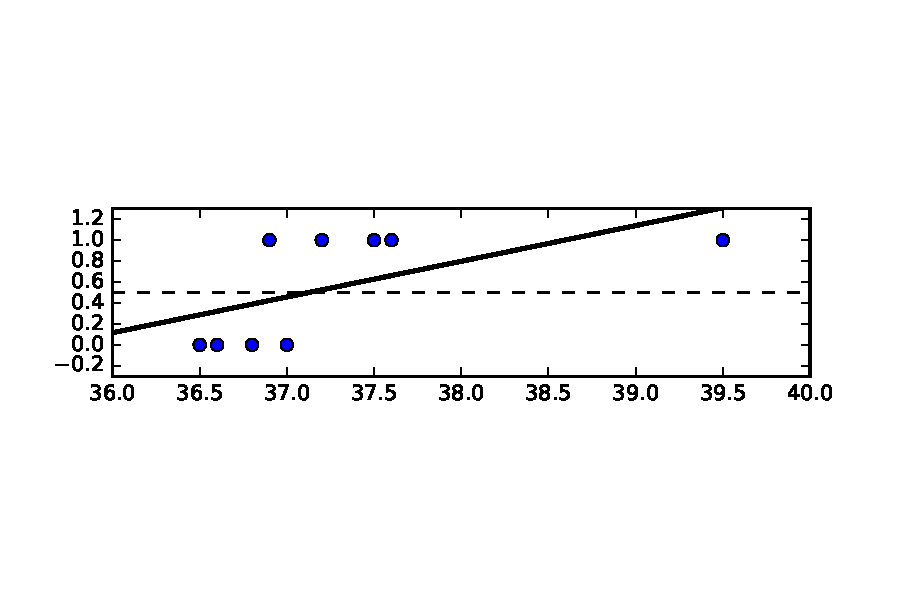
\includegraphics[width=10cm]{figures/class-linreg.pdf}
\caption{An attempt to develop a classifier with a linear regression.}
\label{f:class-linreg}
\end{center}
\end{figure}

In the graphically presented data (Fig.~\ref{f:class-linreg}) we dare to fit the linear function $\hat{y}=f(x)$. We first notice that the range of the function $f(x)$ is inappropriate, since it ranges from $-\infty$ to $\infty$. In the interval of body temperatures around the point $37^{\circ}$, the function has a value between 0 and 1. The question arises how to interpret the estimated value, or how to convert it into probability. Recall that each probability function returns values between 0 and 1, and our linear function is limited to this interval only in a certain range of values of the input attribute. Additional problem is with outliers, or visitors with extreme value of the temperature. If we were to add another case of a patient with a very high temperature to the data, our function would change considerably and shift to the right. We need to instead develop a function that would output the probabilities, soften the output at left and right edges of the data, and then pose the problem in probabilistic and formal terms.

\section{Logistic Function}

Before we continue with a formal introduction of logistic regression, let us introduce a logistic function, a function that converts a real value into an interval from 0 to 1:
\begin{equation}
  g(z) = {1\over 1+e^{-z}}
\end{equation}

\begin{figure}[htbp]
\begin{center}
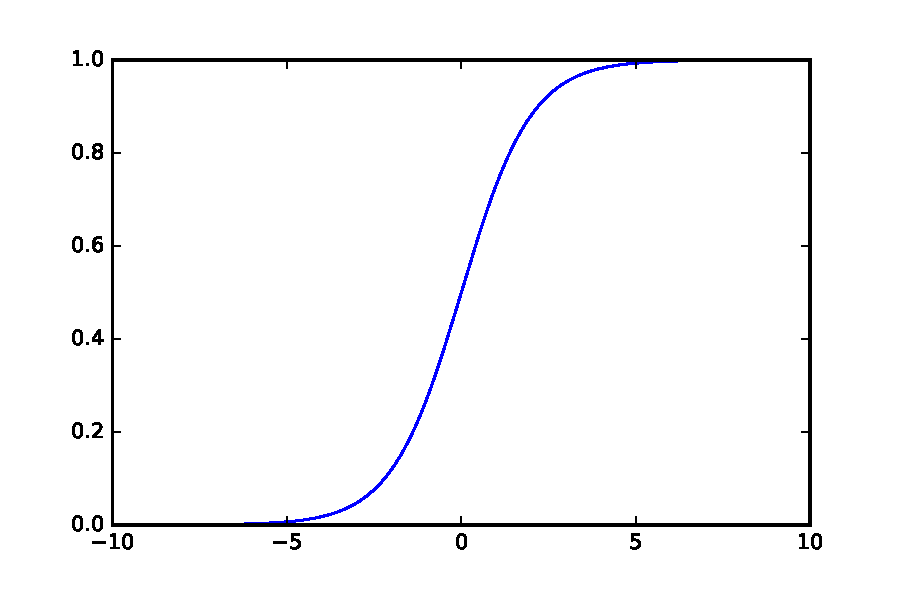
\includegraphics[width=7cm]{figures/logistic.pdf}
\caption{Logistic function.}
\label{f:logistic-function}
\end{center}
\end{figure}

The logistic function (Fig.~\ref{f:logistic-function}) is continuous, monotonic; with $z\to -\infty$ it converges to 0 and with $z\to\infty$ it converges to 1. It derivative exists for all values of its parameter:
\begin{eqnarray}
  \frac{dg(z)}{dz} & = & \frac{d}{dz} \frac{1}{1+e^{-z}} \nonumber \\
  & = & \frac{1}{(1+e^{-z})^2} e^{-z} \nonumber \\
  & = & \frac{1}{1+e^{-z}}\frac{e^{-z}}{1+e^{-z}} \nonumber \\
  & = & \frac{1}{1+e^{-z}}\frac{1+e^{-z}-1}{1+e^{-z}} \nonumber \\
  & = & \frac{1}{1+e^{-z}}\left(1-\frac{1}{1+e^{-z}}\right) \nonumber \\
  & = & g(z)[1-g(z)]
\end{eqnarray}

\section{Likelihood for Logistic Regression}

Following is an equation for a logistic regression model. In the core, this is a linear model, that is, a weighted sum of the values of the input variables. 

\begin{eqnarray}
  f_{\betas}(x) & = & g(\betas_0+\betas_1 x_1+\betas_2 x_2+\ldots\betas_M x_M)
  \nonumber \\
  & = & g(\betas^\tr \x) \nonumber \\
  & = & \frac{1}{1+e^{-\betas^\tr \x}}
  \label{eq:logreg}
\end{eqnarray}

Notice that the linear combination of $\betas$ and values of input variables, when equated to $0$, defines the hyperplane in the feature space. Notice also the all the points that lie on the plane have a value of this function of $0$. The value $0$ is transformed by logistic function to $0.5$. For any other data point that does not lie on the hyperpane the logistic function transforms this value to the value in the interval of $(0.5, 1.0]$ for the points on one side of the hyperplane, or the the value between $(0, 0.5]$ for the points on the other, negative side of the hyperplane. Conveniently, the farther away the point is from the hyperplane, the more to the extremes (0 or 1) will be its value of logistic regression. The hyperplane defined within logistic regression model can thus serve as a decision boundary between two classes.

In what follows, we will use the logistic function so that our model $f_{\betas}(\x)$ returns values between 0 and 1. We will continue to assume that our class variable is two-valued, but assume that its target value is a class marked with $y=1$ and that for it the model $f_{\betas} (\x)$ returns the probability of this class. Notice that the parapeters $\betas$ fully define logistic regression model. Thus, we can write:
\begin{eqnarray}
  p(y=1|\x;\betas) & = & f_{\betas}(x) \\
  p(y=0|\x;\betas) & = & 1-f_{\betas}(x)
\end{eqnarray}
The expression for $p(y=1|\x;\betas) $ therefore gives us the probability that the target class of the data instance described by the vector of attribute values $\x$ is equal to 1. That is, it gives the probability that the independent variable takes the value of $1$ for the data instance described with $\x$, where the model is parametrized with parameters $\betas$. We can combine the two equations into a single one as
\begin{equation}
  p(y|x;\betas) = (f_{\betas}(x))^y(1-f_{\betas}(x))^{1-y}
\label{eq:log-prob}
\end{equation}

The expression for $p(y|\x;\betas) $ in the above equation therefore gives the probability for a certain value of the independent variable and a certain vector of attribute values in the model given by $\betas$. Now imagine that the values of the elements of the vector $\betas$ change. Certainly, in this way, the probability for a given class in a selected case will also change; once this probability will be higher, another time lower. Change in the parameters of the model change the probabilities with which we observe the data from the training set.

Let us now freeze the parameters of the model and compute the joint probability $L(\betas)$, the likelihood, for all the instances in the training set. We assume that the examples from the training set are independent and therefore the probability, with which we observe the values of the classes of particular data instanes described with the vectors $\x$ can be written as the product of the probabilities of individual data instances:
\begin{eqnarray}
  L(\betas) & = & p(\y|\X;\betas) \nonumber\\
  & = & \prod_{i=1}M p(y_i|x_i;\betas) \nonumber\\
  & = & \prod_{i=1}M f_{\betas}(x_i)^{y_i}(1-f_{\betas}(x_i))^{1-y_i}
\end{eqnarray}

Again, just like with the linear regression, we would like to infer the model that maximizes the likelihood. That is, the parameters where we maximize the probability with which the model observes the training set. For convenience of deriving the $\betas$ which maximize the likelihood, we compute its logarithm, and then maximize the log-likelihood:
\begin{eqnarray}
  \ell(\betas) & = & \log L(\betas) \nonumber\\
  & = & \sum_{i=1}M\big[y_i\log f_{\betas}(x_i)+(1-y_i)\log (1-f_{\betas}(x_i)) \big]
\end{eqnarray}

\section{Gradient Descent for Logistic Regression}
We are therefore looking for such $\betas$ that maximizes the log-likelihood $\ell(\betas)$. Since we will use the gradient method, and since $\betas$ is a vector $[\betas_0  \betas_1 \ldots \betas_M] $, we need to calculate the partial derivatives of our criterion function:
\begin{eqnarray}
  \frac{\partial}{\partial\betas_j}\ell(\betas)
  & = & \sum_{i=1}^M \frac{\partial}{\partial\betas_j} \big[y_i\log f_{\betas}(x_i)+(1-y_i)\log (1-f_{\betas}(x_i)) \big] \nonumber \\
  & = & \sum_{i=1}^M \big[y_i\frac{1}{g(\betas^\tr x_i)}-(1-y_i)\frac{1}{1-g(\betas^\tr x_i)} \big]\frac{\partial}{\partial\betas_j}g(\betas^\tr x_i) \nonumber\\
  & = & \sum_{i=1}^M \big[\frac{y_i}{g(\betas^\tr x_i)}-\frac{(1-y_i)}{1-g(\betas^\tr x_i)} \big]g(\betas^\tr x_i)(1-g(\betas^\tr x_i))
  \frac{\partial}{\partial\betas_j}\betas^\tr x_i\nonumber\\
  & = & \sum_{i=1}^M \big[\frac{y_i - g(\betas^\tr x_i)} {g(\betas^\tr x_i)(1-g(\betas^\tr x_i))} \big]g(\betas^\tr x_i)(1-g(\betas^\tr x_i)) x_{ji}\nonumber\\
  & = & \sum_{i=1}^M (y_i-g(\betas^\tr x_i))x_{ji}\nonumber\\
  & = & \sum_{i=1}^M (y_i-f_{\betas}(x_i))x_{ji}
  \label{eq:logreg-grad}
\end{eqnarray}
Very easy! Have we seen such a result or such an equation before? Of course! In linear regression. Partial derivatives are identical to those for linear regression. Of course with a small difference. This time our function $f_{\betas}$ uses the logistic function, while in linear regression $f_{\betas}$ was only the weighted sum of attribute values.

The iterative process using gradient descent to find the parameters of the logistic regression model is identical to that of linear regression. Of course, with the small difference that this time the $ f_{\betas}(x)$ is a logistic regression model. However, we write down the step for refreshing the value of the parameter $ \ theta_j $:
\begin{equation}
  \betas_j\leftarrow\betas_j+\alpha\sum_{i=1}^{m}\big(y_i-f_{\betas}(x_i)\big) x_{ji}
\end{equation}

Again, the $\alpha$ learning rate is typically small for normalized data (e.g., $0.001$).

A warning applies here. The gradient descent approach is slow, and even for medium-sized data, many iterations of correcting the values of the $\betas$ parameters are required. Instead, we typically use optimization techniques that have faster convergence. One of these is the L-BFGS, which is typically used from an accessible Python library.

\printbibliography[heading=subbibliography]
\end{refsection}